\documentclass{standalone}
\usepackage{tikz}
\usetikzlibrary{patterns, positioning}


\begin{document}
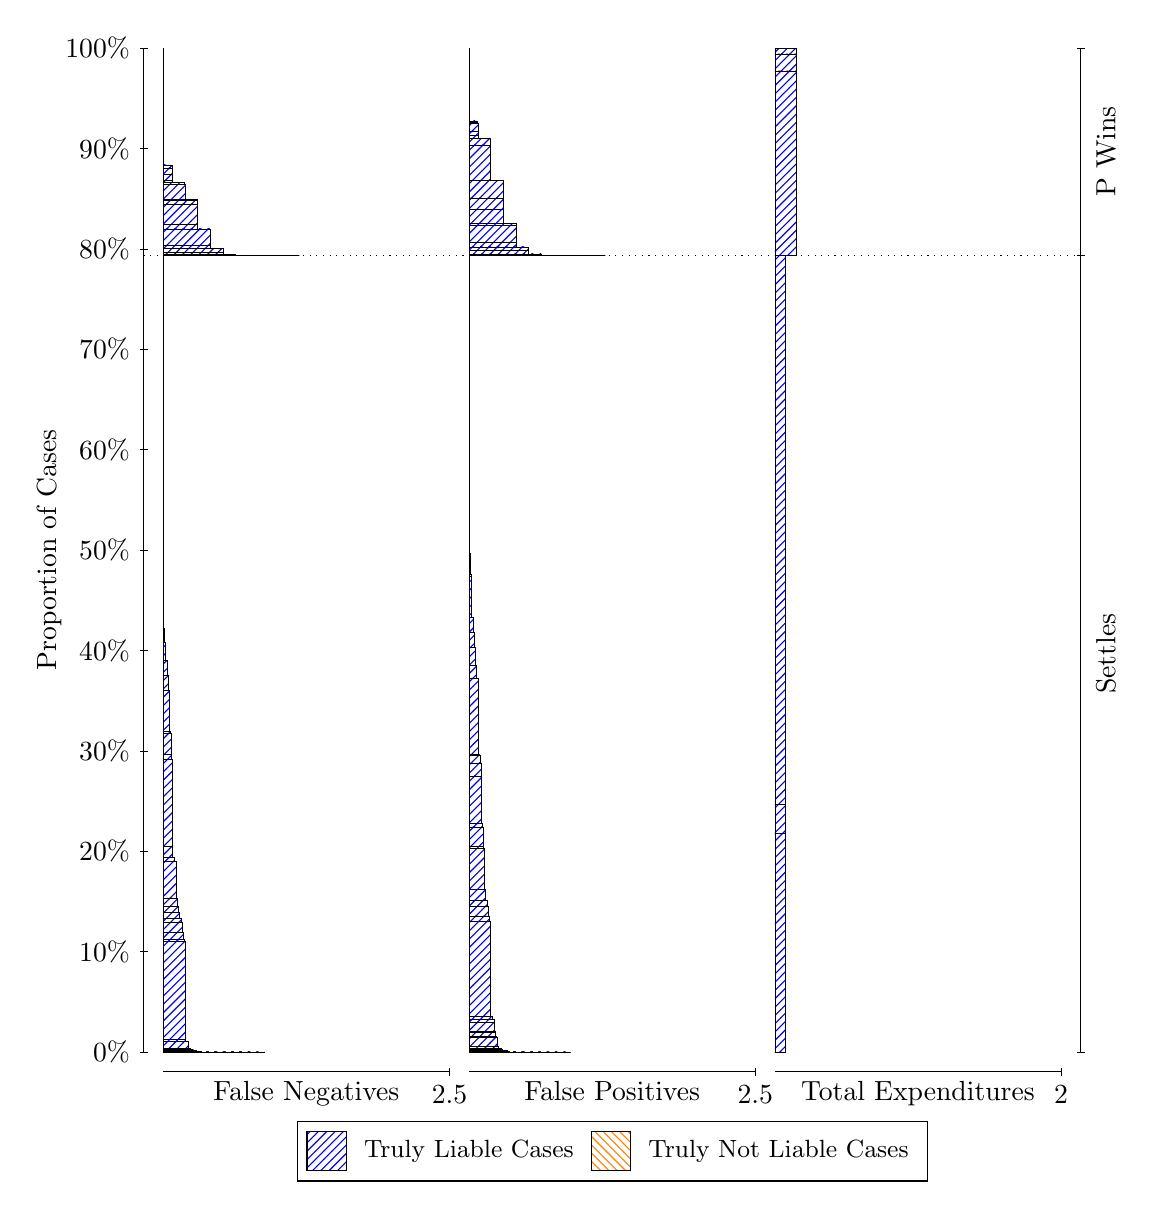
\begin{tikzpicture}
\draw[black, very thin] (1.5,1.75) -- (1.5,14.5);
\node[rotate=90, text=black, anchor=center] at (0.3, 8.125) {Proportion of Cases};
\draw[black, very thin] (1.45,1.75) -- (1.55,1.75);
\node[text=black, anchor=east] at (1.45, 1.75) {0\%};
\draw[black, very thin] (1.45,3.025) -- (1.55,3.025);
\node[text=black, anchor=east] at (1.45, 3.025) {10\%};
\draw[black, very thin] (1.45,4.3) -- (1.55,4.3);
\node[text=black, anchor=east] at (1.45, 4.3) {20\%};
\draw[black, very thin] (1.45,5.575) -- (1.55,5.575);
\node[text=black, anchor=east] at (1.45, 5.575) {30\%};
\draw[black, very thin] (1.45,6.85) -- (1.55,6.85);
\node[text=black, anchor=east] at (1.45, 6.85) {40\%};
\draw[black, very thin] (1.45,8.125) -- (1.55,8.125);
\node[text=black, anchor=east] at (1.45, 8.125) {50\%};
\draw[black, very thin] (1.45,9.4) -- (1.55,9.4);
\node[text=black, anchor=east] at (1.45, 9.4) {60\%};
\draw[black, very thin] (1.45,10.675) -- (1.55,10.675);
\node[text=black, anchor=east] at (1.45, 10.675) {70\%};
\draw[black, very thin] (1.45,11.95) -- (1.55,11.95);
\node[text=black, anchor=east] at (1.45, 11.95) {80\%};
\draw[black, very thin] (1.45,13.225) -- (1.55,13.225);
\node[text=black, anchor=east] at (1.45, 13.225) {90\%};
\draw[black, very thin] (1.45,14.5) -- (1.55,14.5);
\node[text=black, anchor=east] at (1.45, 14.5) {100\%};

\draw[black, very thin] (13.4,1.75) -- (13.4,14.5);
\draw[black, very thin] (13.35,1.75) -- (13.45,1.75);
\node[anchor=west] at (13.35, 1.75) {};
\draw[black, very thin] (13.35,11.866) -- (13.45,11.866);
\node[anchor=west] at (13.35, 11.866) {};
\draw[black, very thin] (13.35,14.5) -- (13.45,14.5);
\node[anchor=west] at (13.35, 14.5) {};

\draw[black, very thin, pattern color=blue, pattern=north east lines] (1.75,1.75) rectangle (3.0398,1.75);
\draw[black, very thin, pattern color=blue, pattern=north east lines] (1.75,1.75) rectangle (2.9672,1.75);
\draw[black, very thin, pattern color=blue, pattern=north east lines] (1.75,1.75) rectangle (2.8945,1.75);
\draw[black, very thin, pattern color=blue, pattern=north east lines] (1.75,1.75) rectangle (2.8784,1.75);
\draw[black, very thin, pattern color=blue, pattern=north east lines] (1.75,1.75) rectangle (2.8218,1.75);
\draw[black, very thin, pattern color=blue, pattern=north east lines] (1.75,1.75) rectangle (2.8057,1.75);
\draw[black, very thin, pattern color=blue, pattern=north east lines] (1.75,1.75) rectangle (2.7492,1.75);
\draw[black, very thin, pattern color=blue, pattern=north east lines] (1.75,1.75) rectangle (2.733,1.75);
\draw[black, very thin, pattern color=blue, pattern=north east lines] (1.75,1.75) rectangle (2.7169,1.75);
\draw[black, very thin, pattern color=blue, pattern=north east lines] (1.75,1.75) rectangle (2.6765,1.75);
\draw[black, very thin, pattern color=blue, pattern=north east lines] (1.75,1.75) rectangle (2.6604,1.75);
\draw[black, very thin, pattern color=blue, pattern=north east lines] (1.75,1.75) rectangle (2.6442,1.75);
\draw[black, very thin, pattern color=blue, pattern=north east lines] (1.75,1.75) rectangle (2.6038,1.75);
\draw[black, very thin, pattern color=blue, pattern=north east lines] (1.75,1.75) rectangle (2.5877,1.75);
\draw[black, very thin, pattern color=blue, pattern=north east lines] (1.75,1.75) rectangle (2.5715,1.75);
\draw[black, very thin, pattern color=blue, pattern=north east lines] (1.75,1.75) rectangle (2.5554,1.75);
\draw[black, very thin, pattern color=blue, pattern=north east lines] (1.75,1.75) rectangle (2.5312,1.75);
\draw[black, very thin, pattern color=blue, pattern=north east lines] (1.75,1.75) rectangle (2.515,1.75);
\draw[black, very thin, pattern color=blue, pattern=north east lines] (1.75,1.75) rectangle (2.4989,1.75);
\draw[black, very thin, pattern color=blue, pattern=north east lines] (1.75,1.75) rectangle (2.4827,1.75);
\draw[black, very thin, pattern color=blue, pattern=north east lines] (1.75,1.75) rectangle (2.4585,1.75);
\draw[black, very thin, pattern color=blue, pattern=north east lines] (1.75,1.75) rectangle (2.4424,1.75);
\draw[black, very thin, pattern color=blue, pattern=north east lines] (1.75,1.75) rectangle (2.4262,1.75);
\draw[black, very thin, pattern color=blue, pattern=north east lines] (1.75,1.75) rectangle (2.4101,1.75);
\draw[black, very thin, pattern color=blue, pattern=north east lines] (1.75,1.75) rectangle (2.3939,1.75);
\draw[black, very thin, pattern color=blue, pattern=north east lines] (1.75,1.75) rectangle (2.3858,1.75);
\draw[black, very thin, pattern color=blue, pattern=north east lines] (1.75,1.75) rectangle (2.3697,1.75);
\draw[black, very thin, pattern color=blue, pattern=north east lines] (1.75,1.75) rectangle (2.3535,1.75);
\draw[black, very thin, pattern color=blue, pattern=north east lines] (1.75,1.75) rectangle (2.3374,1.75);
\draw[black, very thin, pattern color=blue, pattern=north east lines] (1.75,1.75) rectangle (2.3212,1.75);
\draw[black, very thin, pattern color=blue, pattern=north east lines] (1.75,1.75) rectangle (2.3132,1.7502);
\draw[black, very thin, pattern color=blue, pattern=north east lines] (1.75,1.7502) rectangle (2.297,1.7502);
\draw[black, very thin, pattern color=blue, pattern=north east lines] (1.75,1.7502) rectangle (2.2809,1.7502);
\draw[black, very thin, pattern color=blue, pattern=north east lines] (1.75,1.7502) rectangle (2.2647,1.7503);
\draw[black, very thin, pattern color=blue, pattern=north east lines] (1.75,1.7503) rectangle (2.2486,1.7506);
\draw[black, very thin, pattern color=blue, pattern=north east lines] (1.75,1.7506) rectangle (2.2324,1.7541);
\draw[black, very thin, pattern color=blue, pattern=north east lines] (1.75,1.7541) rectangle (2.2244,1.7541);
\draw[black, very thin, pattern color=blue, pattern=north east lines] (1.75,1.7541) rectangle (2.2082,1.7542);
\draw[black, very thin, pattern color=blue, pattern=north east lines] (1.75,1.7542) rectangle (2.1921,1.7548);
\draw[black, very thin, pattern color=blue, pattern=north east lines] (1.75,1.7548) rectangle (2.1759,1.756);
\draw[black, very thin, pattern color=blue, pattern=north east lines] (1.75,1.756) rectangle (2.1678,1.7673);
\draw[black, very thin, pattern color=blue, pattern=north east lines] (1.75,1.7673) rectangle (2.1598,1.7677);
\draw[black, very thin, pattern color=blue, pattern=north east lines] (1.75,1.7677) rectangle (2.1517,1.7745);
\draw[black, very thin, pattern color=blue, pattern=north east lines] (1.75,1.7745) rectangle (2.1355,1.7768);
\draw[black, very thin, pattern color=blue, pattern=north east lines] (1.75,1.7768) rectangle (2.1194,1.7815);
\draw[black, very thin, pattern color=blue, pattern=north east lines] (1.75,1.7815) rectangle (2.1032,1.7863);
\draw[black, very thin, pattern color=blue, pattern=north east lines] (1.75,1.7863) rectangle (2.0871,1.8001);
\draw[black, very thin, pattern color=blue, pattern=north east lines] (1.75,1.8001) rectangle (2.0709,1.8804);
\draw[black, very thin, pattern color=blue, pattern=north east lines] (1.75,1.8804) rectangle (2.0629,1.8806);
\draw[black, very thin, pattern color=blue, pattern=north east lines] (1.75,1.8806) rectangle (2.0467,1.8855);
\draw[black, very thin, pattern color=blue, pattern=north east lines] (1.75,1.8855) rectangle (2.0306,1.9081);
\draw[black, very thin, pattern color=blue, pattern=north east lines] (1.75,1.9081) rectangle (2.0225,3.1603);
\draw[black, very thin, pattern color=blue, pattern=north east lines] (1.75,3.1603) rectangle (2.0144,3.1822);
\draw[black, very thin, pattern color=blue, pattern=north east lines] (1.75,3.1822) rectangle (2.0064,3.2666);
\draw[black, very thin, pattern color=blue, pattern=north east lines] (1.75,3.2666) rectangle (1.9983,3.2731);
\draw[black, very thin, pattern color=blue, pattern=north east lines] (1.75,3.2731) rectangle (1.9902,3.3964);
\draw[black, very thin, pattern color=blue, pattern=north east lines] (1.75,3.3964) rectangle (1.9741,3.4447);
\draw[black, very thin, pattern color=blue, pattern=north east lines] (1.75,3.4447) rectangle (1.9579,3.5192);
\draw[black, very thin, pattern color=blue, pattern=north east lines] (1.75,3.5192) rectangle (1.9418,3.6004);
\draw[black, very thin, pattern color=blue, pattern=north east lines] (1.75,3.6004) rectangle (1.9256,3.7082);
\draw[black, very thin, pattern color=blue, pattern=north east lines] (1.75,3.7082) rectangle (1.9095,4.1659);
\draw[black, very thin, pattern color=blue, pattern=north east lines] (1.75,4.1659) rectangle (1.9014,4.1682);
\draw[black, very thin, pattern color=blue, pattern=north east lines] (1.75,4.1682) rectangle (1.8852,4.2186);
\draw[black, very thin, pattern color=blue, pattern=north east lines] (1.75,4.2186) rectangle (1.8691,4.3646);
\draw[black, very thin, pattern color=blue, pattern=north east lines] (1.75,4.3646) rectangle (1.861,5.4636);
\draw[black, very thin, pattern color=blue, pattern=north east lines] (1.75,5.4636) rectangle (1.8529,5.5316);
\draw[black, very thin, pattern color=blue, pattern=north east lines] (1.75,5.5316) rectangle (1.8449,5.7991);
\draw[black, very thin, pattern color=blue, pattern=north east lines] (1.75,5.7991) rectangle (1.8368,5.8247);
\draw[black, very thin, pattern color=blue, pattern=north east lines] (1.75,5.8247) rectangle (1.8287,6.3462);
\draw[black, very thin, pattern color=blue, pattern=north east lines] (1.75,6.3462) rectangle (1.8126,6.5388);
\draw[black, very thin, pattern color=blue, pattern=north east lines] (1.75,6.5388) rectangle (1.7964,6.7257);
\draw[black, very thin, pattern color=blue, pattern=north east lines] (1.75,6.7257) rectangle (1.7803,6.9556);
\draw[black, very thin, pattern color=blue, pattern=north east lines] (1.75,6.9556) rectangle (1.7641,7.1261);
\draw[black, very thin, pattern color=orange, pattern=north west lines] (1.75,7.1261) rectangle (1.75,7.1261);
\draw[black, very thin, pattern color=blue, pattern=north east lines] (1.75,7.1261) rectangle (1.75,11.866);
\draw[black, very thin, pattern color=blue, pattern=north east lines] (1.75,11.866) rectangle (3.4758,11.866);
\draw[black, very thin, pattern color=blue, pattern=north east lines] (1.75,11.866) rectangle (3.3144,11.866);
\draw[black, very thin, pattern color=blue, pattern=north east lines] (1.75,11.866) rectangle (3.1529,11.866);
\draw[black, very thin, pattern color=blue, pattern=north east lines] (1.75,11.866) rectangle (3.1529,11.866);
\draw[black, very thin, pattern color=blue, pattern=north east lines] (1.75,11.866) rectangle (2.9914,11.866);
\draw[black, very thin, pattern color=blue, pattern=north east lines] (1.75,11.866) rectangle (2.9914,11.866);
\draw[black, very thin, pattern color=blue, pattern=north east lines] (1.75,11.866) rectangle (2.8299,11.867);
\draw[black, very thin, pattern color=blue, pattern=north east lines] (1.75,11.867) rectangle (2.8259,11.867);
\draw[black, very thin, pattern color=blue, pattern=north east lines] (1.75,11.867) rectangle (2.6684,11.88);
\draw[black, very thin, pattern color=blue, pattern=north east lines] (1.75,11.88) rectangle (2.6644,11.88);
\draw[black, very thin, pattern color=blue, pattern=north east lines] (1.75,11.88) rectangle (2.5069,11.904);
\draw[black, very thin, pattern color=blue, pattern=north east lines] (1.75,11.904) rectangle (2.5069,11.956);
\draw[black, very thin, pattern color=blue, pattern=north east lines] (1.75,11.956) rectangle (2.5029,11.956);
\draw[black, very thin, pattern color=blue, pattern=north east lines] (1.75,11.956) rectangle (2.5029,11.956);
\draw[black, very thin, pattern color=blue, pattern=north east lines] (1.75,11.956) rectangle (2.3455,11.993);
\draw[black, very thin, pattern color=blue, pattern=north east lines] (1.75,11.993) rectangle (2.3455,12.204);
\draw[black, very thin, pattern color=blue, pattern=north east lines] (1.75,12.204) rectangle (2.3414,12.204);
\draw[black, very thin, pattern color=blue, pattern=north east lines] (1.75,12.204) rectangle (2.3414,12.204);
\draw[black, very thin, pattern color=blue, pattern=north east lines] (1.75,12.204) rectangle (2.184,12.26);
\draw[black, very thin, pattern color=blue, pattern=north east lines] (1.75,12.26) rectangle (2.184,12.52);
\draw[black, very thin, pattern color=blue, pattern=north east lines] (1.75,12.52) rectangle (2.184,12.572);
\draw[black, very thin, pattern color=blue, pattern=north east lines] (1.75,12.572) rectangle (2.1799,12.573);
\draw[black, very thin, pattern color=blue, pattern=north east lines] (1.75,12.573) rectangle (2.1799,12.573);
\draw[black, very thin, pattern color=blue, pattern=north east lines] (1.75,12.573) rectangle (2.1799,12.573);
\draw[black, very thin, pattern color=blue, pattern=north east lines] (1.75,12.573) rectangle (2.0225,12.766);
\draw[black, very thin, pattern color=blue, pattern=north east lines] (1.75,12.766) rectangle (2.0185,12.767);
\draw[black, very thin, pattern color=blue, pattern=north east lines] (1.75,12.767) rectangle (2.0185,12.791);
\draw[black, very thin, pattern color=blue, pattern=north east lines] (1.75,12.791) rectangle (1.861,12.818);
\draw[black, very thin, pattern color=blue, pattern=north east lines] (1.75,12.818) rectangle (1.861,12.819);
\draw[black, very thin, pattern color=blue, pattern=north east lines] (1.75,12.819) rectangle (1.857,12.9);
\draw[black, very thin, pattern color=blue, pattern=north east lines] (1.75,12.9) rectangle (1.857,12.978);
\draw[black, very thin, pattern color=blue, pattern=north east lines] (1.75,12.978) rectangle (1.857,13.016);
\draw[black, very thin, pattern color=orange, pattern=north west lines] (1.75,13.016) rectangle (1.75,13.016);
\draw[black, very thin, pattern color=blue, pattern=north east lines] (1.75,13.016) rectangle (1.75,14.5);
\draw[black, very thin, pattern color=orange, pattern=north west lines] (5.6333,1.75) rectangle (6.9232,1.75);
\draw[black, very thin, pattern color=blue, pattern=north east lines] (5.6333,1.75) rectangle (6.9232,1.75);
\draw[black, very thin, pattern color=orange, pattern=north west lines] (5.6333,1.75) rectangle (6.7778,1.75);
\draw[black, very thin, pattern color=blue, pattern=north east lines] (5.6333,1.75) rectangle (6.7778,1.75);
\draw[black, very thin, pattern color=blue, pattern=north east lines] (5.6333,1.75) rectangle (6.7617,1.75);
\draw[black, very thin, pattern color=orange, pattern=north west lines] (5.6333,1.75) rectangle (6.6325,1.75);
\draw[black, very thin, pattern color=blue, pattern=north east lines] (5.6333,1.75) rectangle (6.6325,1.75);
\draw[black, very thin, pattern color=blue, pattern=north east lines] (5.6333,1.75) rectangle (6.6164,1.75);
\draw[black, very thin, pattern color=blue, pattern=north east lines] (5.6333,1.75) rectangle (6.6002,1.75);
\draw[black, very thin, pattern color=orange, pattern=north west lines] (5.6333,1.75) rectangle (6.5598,1.75);
\draw[black, very thin, pattern color=blue, pattern=north east lines] (5.6333,1.75) rectangle (6.5598,1.75);
\draw[black, very thin, pattern color=orange, pattern=north west lines] (5.6333,1.75) rectangle (6.4872,1.75);
\draw[black, very thin, pattern color=blue, pattern=north east lines] (5.6333,1.75) rectangle (6.4872,1.75);
\draw[black, very thin, pattern color=blue, pattern=north east lines] (5.6333,1.75) rectangle (6.471,1.75);
\draw[black, very thin, pattern color=blue, pattern=north east lines] (5.6333,1.75) rectangle (6.4549,1.75);
\draw[black, very thin, pattern color=blue, pattern=north east lines] (5.6333,1.75) rectangle (6.4387,1.75);
\draw[black, very thin, pattern color=orange, pattern=north west lines] (5.6333,1.75) rectangle (6.4145,1.75);
\draw[black, very thin, pattern color=blue, pattern=north east lines] (5.6333,1.75) rectangle (6.4145,1.75);
\draw[black, very thin, pattern color=blue, pattern=north east lines] (5.6333,1.75) rectangle (6.3984,1.75);
\draw[black, very thin, pattern color=orange, pattern=north west lines] (5.6333,1.75) rectangle (6.3418,1.75);
\draw[black, very thin, pattern color=blue, pattern=north east lines] (5.6333,1.75) rectangle (6.3418,1.75);
\draw[black, very thin, pattern color=blue, pattern=north east lines] (5.6333,1.75) rectangle (6.3257,1.75);
\draw[black, very thin, pattern color=blue, pattern=north east lines] (5.6333,1.75) rectangle (6.3095,1.7501);
\draw[black, very thin, pattern color=blue, pattern=north east lines] (5.6333,1.7501) rectangle (6.2934,1.7501);
\draw[black, very thin, pattern color=blue, pattern=north east lines] (5.6333,1.7501) rectangle (6.2772,1.7501);
\draw[black, very thin, pattern color=orange, pattern=north west lines] (5.6333,1.7501) rectangle (6.2692,1.7501);
\draw[black, very thin, pattern color=blue, pattern=north east lines] (5.6333,1.7501) rectangle (6.2692,1.7501);
\draw[black, very thin, pattern color=blue, pattern=north east lines] (5.6333,1.7501) rectangle (6.253,1.7502);
\draw[black, very thin, pattern color=blue, pattern=north east lines] (5.6333,1.7502) rectangle (6.2369,1.7502);
\draw[black, very thin, pattern color=orange, pattern=north west lines] (5.6333,1.7502) rectangle (6.1965,1.7502);
\draw[black, very thin, pattern color=blue, pattern=north east lines] (5.6333,1.7502) rectangle (6.1965,1.7506);
\draw[black, very thin, pattern color=blue, pattern=north east lines] (5.6333,1.7506) rectangle (6.1804,1.7507);
\draw[black, very thin, pattern color=blue, pattern=north east lines] (5.6333,1.7507) rectangle (6.1642,1.7512);
\draw[black, very thin, pattern color=blue, pattern=north east lines] (5.6333,1.7512) rectangle (6.1481,1.7569);
\draw[black, very thin, pattern color=blue, pattern=north east lines] (5.6333,1.7569) rectangle (6.1319,1.7593);
\draw[black, very thin, pattern color=orange, pattern=north west lines] (5.6333,1.7593) rectangle (6.1238,1.7593);
\draw[black, very thin, pattern color=blue, pattern=north east lines] (5.6333,1.7593) rectangle (6.1238,1.7597);
\draw[black, very thin, pattern color=blue, pattern=north east lines] (5.6333,1.7597) rectangle (6.1158,1.7654);
\draw[black, very thin, pattern color=blue, pattern=north east lines] (5.6333,1.7654) rectangle (6.1077,1.767);
\draw[black, very thin, pattern color=blue, pattern=north east lines] (5.6333,1.767) rectangle (6.0915,1.77);
\draw[black, very thin, pattern color=blue, pattern=north east lines] (5.6333,1.77) rectangle (6.0754,1.7702);
\draw[black, very thin, pattern color=orange, pattern=north west lines] (5.6333,1.7702) rectangle (6.0512,1.7702);
\draw[black, very thin, pattern color=blue, pattern=north east lines] (5.6333,1.7702) rectangle (6.0512,1.7807);
\draw[black, very thin, pattern color=blue, pattern=north east lines] (5.6333,1.7807) rectangle (6.035,1.7939);
\draw[black, very thin, pattern color=blue, pattern=north east lines] (5.6333,1.7939) rectangle (6.0189,1.7986);
\draw[black, very thin, pattern color=blue, pattern=north east lines] (5.6333,1.7986) rectangle (6.0027,1.8192);
\draw[black, very thin, pattern color=blue, pattern=north east lines] (5.6333,1.8192) rectangle (5.9866,1.9387);
\draw[black, very thin, pattern color=orange, pattern=north west lines] (5.6333,1.9387) rectangle (5.9785,1.9387);
\draw[black, very thin, pattern color=blue, pattern=north east lines] (5.6333,1.9387) rectangle (5.9785,1.9489);
\draw[black, very thin, pattern color=blue, pattern=north east lines] (5.6333,1.9489) rectangle (5.9704,2.0021);
\draw[black, very thin, pattern color=blue, pattern=north east lines] (5.6333,2.0021) rectangle (5.9624,2.0089);
\draw[black, very thin, pattern color=blue, pattern=north east lines] (5.6333,2.0089) rectangle (5.9543,2.1301);
\draw[black, very thin, pattern color=blue, pattern=north east lines] (5.6333,2.1301) rectangle (5.9462,2.1643);
\draw[black, very thin, pattern color=blue, pattern=north east lines] (5.6333,2.1643) rectangle (5.9301,2.2043);
\draw[black, very thin, pattern color=blue, pattern=north east lines] (5.6333,2.2043) rectangle (5.9139,2.2064);
\draw[black, very thin, pattern color=orange, pattern=north west lines] (5.6333,2.2064) rectangle (5.9058,2.2064);
\draw[black, very thin, pattern color=blue, pattern=north east lines] (5.6333,2.2064) rectangle (5.9058,3.4083);
\draw[black, very thin, pattern color=blue, pattern=north east lines] (5.6333,3.4083) rectangle (5.8897,3.4774);
\draw[black, very thin, pattern color=blue, pattern=north east lines] (5.6333,3.4774) rectangle (5.8735,3.5962);
\draw[black, very thin, pattern color=blue, pattern=north east lines] (5.6333,3.5962) rectangle (5.8574,3.6707);
\draw[black, very thin, pattern color=blue, pattern=north east lines] (5.6333,3.6707) rectangle (5.8412,3.8183);
\draw[black, very thin, pattern color=blue, pattern=north east lines] (5.6333,3.8183) rectangle (5.8251,4.3364);
\draw[black, very thin, pattern color=blue, pattern=north east lines] (5.6333,4.3364) rectangle (5.817,4.3625);
\draw[black, very thin, pattern color=blue, pattern=north east lines] (5.6333,4.3625) rectangle (5.8089,4.6082);
\draw[black, very thin, pattern color=blue, pattern=north east lines] (5.6333,4.6082) rectangle (5.8009,4.6509);
\draw[black, very thin, pattern color=blue, pattern=north east lines] (5.6333,4.6509) rectangle (5.7928,5.2571);
\draw[black, very thin, pattern color=blue, pattern=north east lines] (5.6333,5.2571) rectangle (5.7847,5.421);
\draw[black, very thin, pattern color=blue, pattern=north east lines] (5.6333,5.421) rectangle (5.7686,5.523);
\draw[black, very thin, pattern color=blue, pattern=north east lines] (5.6333,5.523) rectangle (5.7524,5.5283);
\draw[black, very thin, pattern color=blue, pattern=north east lines] (5.6333,5.5283) rectangle (5.7444,6.4899);
\draw[black, very thin, pattern color=blue, pattern=north east lines] (5.6333,6.4899) rectangle (5.7282,6.6604);
\draw[black, very thin, pattern color=blue, pattern=north east lines] (5.6333,6.6604) rectangle (5.7121,6.8903);
\draw[black, very thin, pattern color=blue, pattern=north east lines] (5.6333,6.8903) rectangle (5.6959,7.0773);
\draw[black, very thin, pattern color=blue, pattern=north east lines] (5.6333,7.0773) rectangle (5.6798,7.2698);
\draw[black, very thin, pattern color=blue, pattern=north east lines] (5.6333,7.2698) rectangle (5.6636,7.7913);
\draw[black, very thin, pattern color=blue, pattern=north east lines] (5.6333,7.7913) rectangle (5.6555,7.8169);
\draw[black, very thin, pattern color=blue, pattern=north east lines] (5.6333,7.8169) rectangle (5.6475,8.0844);
\draw[black, very thin, pattern color=blue, pattern=north east lines] (5.6333,8.0844) rectangle (5.6394,8.1524);
\draw[black, very thin, pattern color=blue, pattern=north east lines] (5.6333,8.1524) rectangle (5.6333,11.866);
\draw[black, very thin, pattern color=orange, pattern=north west lines] (5.6333,11.866) rectangle (7.3592,11.866);
\draw[black, very thin, pattern color=blue, pattern=north east lines] (5.6333,11.866) rectangle (7.3592,11.866);
\draw[black, very thin, pattern color=orange, pattern=north west lines] (5.6333,11.866) rectangle (7.1977,11.866);
\draw[black, very thin, pattern color=blue, pattern=north east lines] (5.6333,11.866) rectangle (7.1977,11.866);
\draw[black, very thin, pattern color=orange, pattern=north west lines] (5.6333,11.866) rectangle (7.0362,11.866);
\draw[black, very thin, pattern color=blue, pattern=north east lines] (5.6333,11.866) rectangle (7.0362,11.866);
\draw[black, very thin, pattern color=blue, pattern=north east lines] (5.6333,11.866) rectangle (7.0362,11.866);
\draw[black, very thin, pattern color=blue, pattern=north east lines] (5.6333,11.866) rectangle (6.8747,11.866);
\draw[black, very thin, pattern color=orange, pattern=north west lines] (5.6333,11.866) rectangle (6.8747,11.866);
\draw[black, very thin, pattern color=blue, pattern=north east lines] (5.6333,11.866) rectangle (6.8747,11.866);
\draw[black, very thin, pattern color=orange, pattern=north west lines] (5.6333,11.866) rectangle (6.7132,11.866);
\draw[black, very thin, pattern color=blue, pattern=north east lines] (5.6333,11.866) rectangle (6.7132,11.868);
\draw[black, very thin, pattern color=orange, pattern=north west lines] (5.6333,11.868) rectangle (6.5518,11.868);
\draw[black, very thin, pattern color=blue, pattern=north east lines] (5.6333,11.868) rectangle (6.5518,11.885);
\draw[black, very thin, pattern color=blue, pattern=north east lines] (5.6333,11.885) rectangle (6.3903,11.932);
\draw[black, very thin, pattern color=orange, pattern=north west lines] (5.6333,11.932) rectangle (6.3903,11.932);
\draw[black, very thin, pattern color=blue, pattern=north east lines] (5.6333,11.932) rectangle (6.3903,11.975);
\draw[black, very thin, pattern color=orange, pattern=north west lines] (5.6333,11.975) rectangle (6.3862,11.975);
\draw[black, very thin, pattern color=blue, pattern=north east lines] (5.6333,11.975) rectangle (6.3862,11.975);
\draw[black, very thin, pattern color=blue, pattern=north east lines] (5.6333,11.975) rectangle (6.2288,12.029);
\draw[black, very thin, pattern color=orange, pattern=north west lines] (5.6333,12.029) rectangle (6.2288,12.029);
\draw[black, very thin, pattern color=blue, pattern=north east lines] (5.6333,12.029) rectangle (6.2288,12.243);
\draw[black, very thin, pattern color=blue, pattern=north east lines] (5.6333,12.243) rectangle (6.2288,12.269);
\draw[black, very thin, pattern color=blue, pattern=north east lines] (5.6333,12.269) rectangle (6.2248,12.269);
\draw[black, very thin, pattern color=orange, pattern=north west lines] (5.6333,12.269) rectangle (6.2248,12.269);
\draw[black, very thin, pattern color=blue, pattern=north east lines] (5.6333,12.269) rectangle (6.2248,12.269);
\draw[black, very thin, pattern color=blue, pattern=north east lines] (5.6333,12.269) rectangle (6.0673,12.453);
\draw[black, very thin, pattern color=blue, pattern=north east lines] (5.6333,12.453) rectangle (6.0673,12.598);
\draw[black, very thin, pattern color=blue, pattern=north east lines] (5.6333,12.598) rectangle (6.0673,12.82);
\draw[black, very thin, pattern color=blue, pattern=north east lines] (5.6333,12.82) rectangle (6.0633,12.82);
\draw[black, very thin, pattern color=orange, pattern=north west lines] (5.6333,12.82) rectangle (6.0633,12.82);
\draw[black, very thin, pattern color=blue, pattern=north east lines] (5.6333,12.82) rectangle (6.0633,12.82);
\draw[black, very thin, pattern color=blue, pattern=north east lines] (5.6333,12.82) rectangle (5.9058,13.269);
\draw[black, very thin, pattern color=blue, pattern=north east lines] (5.6333,13.269) rectangle (5.9058,13.35);
\draw[black, very thin, pattern color=blue, pattern=north east lines] (5.6333,13.35) rectangle (5.9018,13.35);
\draw[black, very thin, pattern color=orange, pattern=north west lines] (5.6333,13.35) rectangle (5.9018,13.35);
\draw[black, very thin, pattern color=blue, pattern=north east lines] (5.6333,13.35) rectangle (5.9018,13.35);
\draw[black, very thin, pattern color=blue, pattern=north east lines] (5.6333,13.35) rectangle (5.7444,13.388);
\draw[black, very thin, pattern color=blue, pattern=north east lines] (5.6333,13.388) rectangle (5.7444,13.448);
\draw[black, very thin, pattern color=blue, pattern=north east lines] (5.6333,13.448) rectangle (5.7444,13.547);
\draw[black, very thin, pattern color=blue, pattern=north east lines] (5.6333,13.547) rectangle (5.7403,13.548);
\draw[black, very thin, pattern color=blue, pattern=north east lines] (5.6333,13.548) rectangle (5.7403,13.558);
\draw[black, very thin, pattern color=orange, pattern=north west lines] (5.6333,13.558) rectangle (5.7403,13.558);
\draw[black, very thin, pattern color=blue, pattern=north east lines] (5.6333,13.558) rectangle (5.7403,13.575);
\draw[black, very thin, pattern color=orange, pattern=north west lines] (5.6333,13.575) rectangle (5.6333,13.575);
\draw[black, very thin, pattern color=blue, pattern=north east lines] (5.6333,13.575) rectangle (5.6333,14.5);
\draw[black, very thin, pattern color=orange, pattern=north west lines] (9.5167,1.75) rectangle (9.6529,1.75);
\draw[black, very thin, pattern color=blue, pattern=north east lines] (9.5167,1.75) rectangle (9.6529,4.5236);
\draw[black, very thin, pattern color=orange, pattern=north west lines] (9.5167,4.5236) rectangle (9.6529,4.5236);
\draw[black, very thin, pattern color=blue, pattern=north east lines] (9.5167,4.5236) rectangle (9.6529,4.8956);
\draw[black, very thin, pattern color=orange, pattern=north west lines] (9.5167,4.8956) rectangle (9.6529,4.8956);
\draw[black, very thin, pattern color=blue, pattern=north east lines] (9.5167,4.8956) rectangle (9.6529,11.866);
\draw[black, very thin, pattern color=orange, pattern=north west lines] (9.5167,11.866) rectangle (9.7892,11.866);
\draw[black, very thin, pattern color=blue, pattern=north east lines] (9.5167,11.866) rectangle (9.7892,14.211);
\draw[black, very thin, pattern color=orange, pattern=north west lines] (9.5167,14.211) rectangle (9.7892,14.211);
\draw[black, very thin, pattern color=blue, pattern=north east lines] (9.5167,14.211) rectangle (9.7892,14.426);
\draw[black, very thin, pattern color=orange, pattern=north west lines] (9.5167,14.426) rectangle (9.7892,14.426);
\draw[black, very thin, pattern color=blue, pattern=north east lines] (9.5167,14.426) rectangle (9.7892,14.5);
\draw[black, dotted] (1.5,11.866) -- (13.4,11.866);
\draw[black, very thin] (1.75,1.5) -- (5.3833,1.5);
\node[text=black, anchor=north] at (3.5667, 1.5) {False Negatives};
\draw[black, very thin] (5.3833,1.45) -- (5.3833,1.55);
\node[text=black, anchor=north] at (5.3833, 1.45) {2.5};

\draw[black, very thin] (5.6333,1.5) -- (9.2667,1.5);
\node[text=black, anchor=north] at (7.45, 1.5) {False Positives};
\draw[black, very thin] (9.2667,1.45) -- (9.2667,1.55);
\node[text=black, anchor=north] at (9.2667, 1.45) {2.5};

\draw[black, very thin] (9.5167,1.5) -- (13.15,1.5);
\node[text=black, anchor=north] at (11.333, 1.5) {Total Expenditures};
\draw[black, very thin] (13.15,1.45) -- (13.15,1.55);
\node[text=black, anchor=north] at (13.15, 1.45) {2};

\node[text=black, centered, rotate=90] at (13.72, 6.808) {Settles};
\node[text=black, centered, rotate=90] at (13.72, 13.183) {P Wins};

\draw (7.449999999999999,1.5) node[draw=none] (baseCoordinate) {};
\begin{scope}[align=center]
        \matrix[scale=0.5, draw=black, below=0.5cm of baseCoordinate, nodes={draw}, column sep=0.1cm]{
            \node[rectangle, draw, minimum width=0.5cm, minimum height=0.5cm, pattern color=blue, pattern=north east lines] {}; &
            \node[draw=none, font=\small, text=black] (B) {Truly Liable Cases}; &
            \node[rectangle, draw, minimum width=0.5cm, minimum height=0.5cm, pattern color=orange, pattern=north west lines] {}; &
            \node[draw=none, font=\small, text=black] (B) {Truly Not Liable Cases}; \\
            };
\end{scope}

\end{tikzpicture}
\end{document}